
%\newgeometry{left=1.5in,right=1.5in,top=0.20in,bottom=1.0in}

\begin{figure*}

\mbox{\hspace*{0.0\textwidth}
\begin{subfigure}[b]{0.55\textwidth}
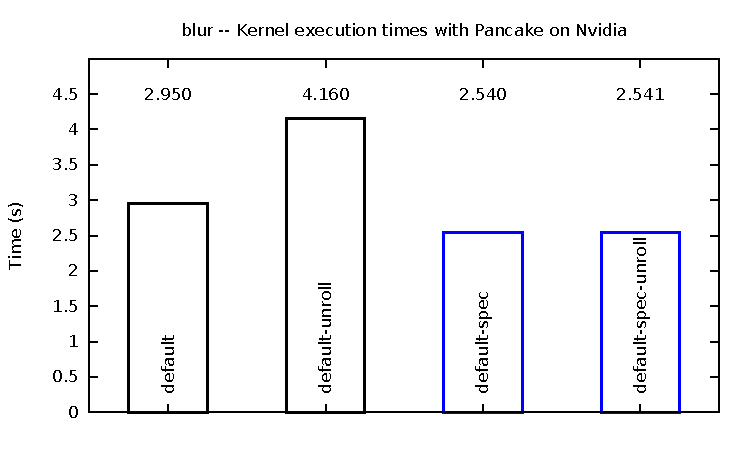
\includegraphics[width=3.0in]{charts/nvidia/blur-exec}
\end{subfigure}
\begin{subfigure}[b]{0.55\textwidth}
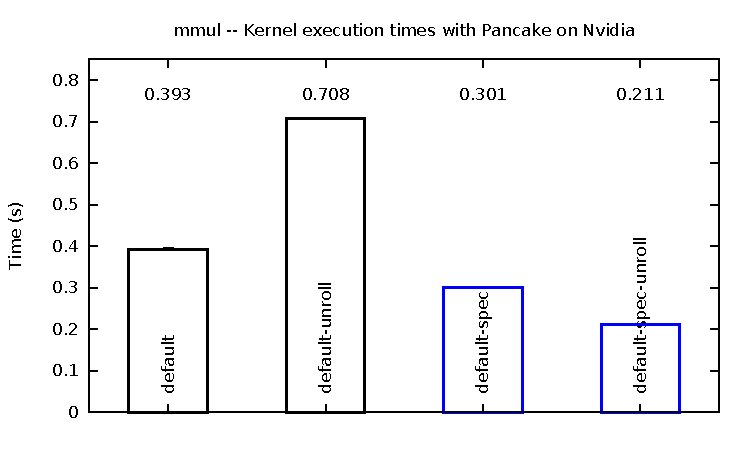
\includegraphics[width=3.0in]{charts/nvidia/mmul-exec}
\end{subfigure}}

\mbox{\hspace*{0.0\textwidth}
\begin{subfigure}[b]{0.55\textwidth}
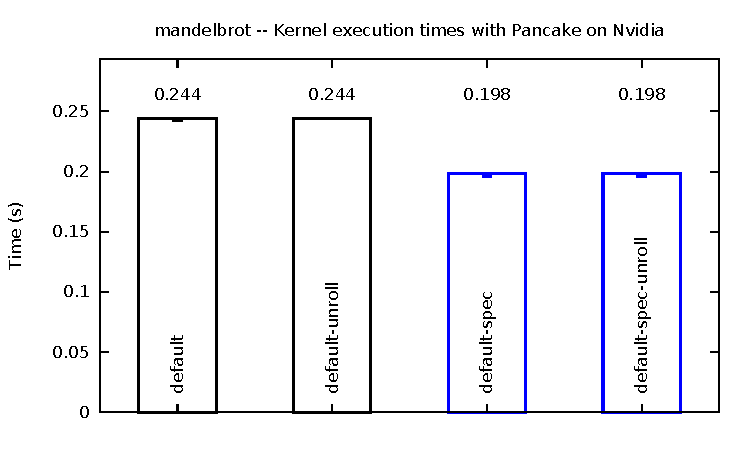
\includegraphics[width=3.0in]{charts/nvidia/mandelbrot-exec}
\end{subfigure}
\begin{subfigure}[b]{0.55\textwidth}
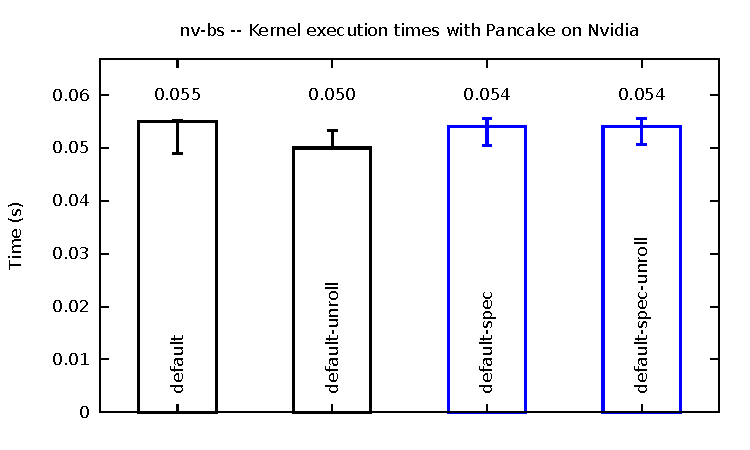
\includegraphics[width=3.0in]{charts/nvidia/nv-bs-exec}
\end{subfigure}}

\mbox{\hspace*{0.0\textwidth}
\begin{subfigure}[b]{0.55\textwidth}
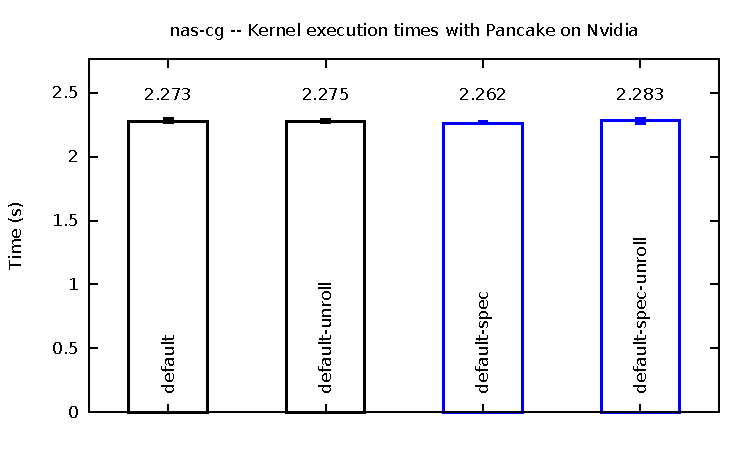
\includegraphics[width=3.0in]{charts/nvidia/nas-cg-exec}
\end{subfigure}
\begin{subfigure}[b]{0.55\textwidth}
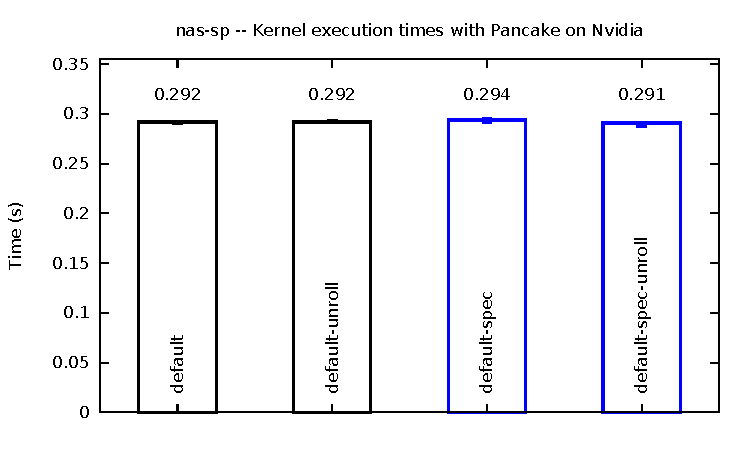
\includegraphics[width=3.0in]{charts/nvidia/nas-sp-exec}
\end{subfigure}}

\mbox{\hspace*{0.0\textwidth}
\begin{subfigure}[b]{0.55\textwidth}
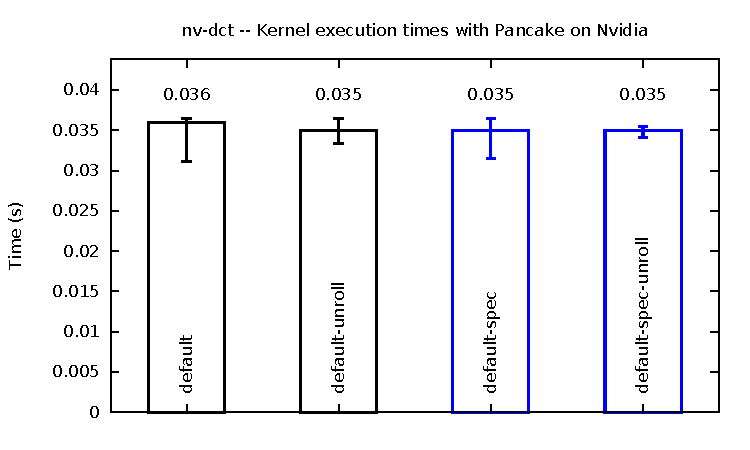
\includegraphics[width=3.0in]{charts/nvidia/nv-dct-exec}
\end{subfigure}
\begin{subfigure}[b]{0.55\textwidth}
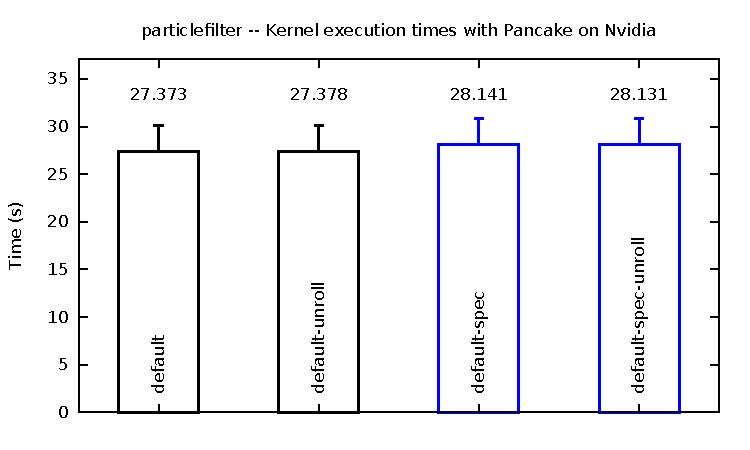
\includegraphics[width=3.0in]{charts/nvidia/particlefilter-exec}
\end{subfigure}}

\caption{\label{pancake-nvidia-table} Benchmark Timings for Pancake on Nvidia GTX 650 Ti}
\end{figure*}

%\restoregeometry

